\documentclass[sigplan,screen]{acmart}

%\usepackage{listings}
\usepackage{xspace}
\newcommand{\lin}[1]{(\emph{ln. #1}\xspace)}
\newcommand{\dapp}{\emph{dapp}\xspace}
\newcommand{\dapps}{\emph{dapps}\xspace}

\setcopyright{acmcopyright}
\copyrightyear{2018}
\acmYear{2018}
\acmDOI{10.1145/1122445.1122456}

\acmConference[REBLS '21]{REBLS '21: ACM Workshop on Reactive and Event-Based Languages and Systems}{June 03--05, 2018}{Chicago, IL}
\acmBooktitle{REBLS '21: ACM Workshop on Reactive and Event-Based Languages and Systems, June 03--05, 2018, Chicago, IL}
\acmPrice{15.00}
\acmISBN{978-1-4503-XXXX-X/18/06}

%\acmSubmissionID{123-A56-BU3}
%\citestyle{acmauthoryear}

\begin{document}

\title{Deterministic Distributed Interactive Applications}

\author{Francisco Sant'Anna}
\email{francisco@ime.uerj.br}
%\orcid{1234-5678-9012}
\affiliation{%
  \institution{Rio de Janeiro State University (UERJ)}
  \country{Brazil}
}

\author{Rodrigo Santos}
\email{rodrim.c@gmail.com}
\affiliation{%
  \institution{Microsoft}
  \country{Brazil}
}

\author{Noemi Rodriguez}
\email{noemi@inf.puc-rio.br}
\affiliation{%
  \institution{PUC-Rio}
  \country{Brazil}
}

%\renewcommand{\shortauthors}{Trovato and Tobin, et al.}

\begin{abstract}
A program is deterministic if multiple re-executions with the same order of
inputs always lead to the same state.
For a given deterministic program, it should even be possible to provide the
same set of inputs to concurrent instances and observe identical behavior in
real time.
%
In this work, we guarantee real-time reproducibility in a distributed setting.
Multiple instances of the same application can broadcast asynchronous inputs
and yet conform to identical behavior.
Collaborative networked applications, such as watch parties, document editing,
and video games can benefit of this approach.
%
Using a standard event-driven API to wait and emit events, programmers write
code as if the application executes in a single machine.
Our middleware intercepts event generation and synchronizes all instances so
that receipt is identically reproducible.
Not only distributed applications benefit of determinism but also development
and testing can be done in a single instance with the same guarantees.
\end{abstract}

\begin{comment}
\begin{CCSXML}
<ccs2012>
 <concept>
  <concept_id>10003033.10003083.10003095</concept_id>
  <concept_desc>Networks~Network reliability</concept_desc>
  <concept_significance>100</concept_significance>
 </concept>
</ccs2012>
\end{CCSXML}
\ccsdesc[100]{Networks~Network reliability}
\end{comment}

%\keywords{globally-asynchronous locally-synchronous, synchronous programming}
\keywords{TODO}

\maketitle

\section{Introduction}

Deterministic programs are easier to understand, test, and verify~\cite{det}.
Considering unpredictable user interactions, a program is deterministic if
re-execution with the same order and timing of inputs always leads to the same
state.
With such reproducibility property, multiple re-executions are
indistinguishable from one another.
Considering now distribution, it should even be possible to provide the same
set of inputs to concurrent instances of a deterministic program and observe
identical behavior in real time.

In this work, our goal is to guarantee the real-time reproducibility property
in a distributed setting.
Mirrored instances of the same application running in different machines can
broadcast asynchronous inputs to each other and yet conform to
identical behavior.
Hence, our focus is on \emph{symmetric distributed applications}, instead of
machines playing different roles in the network.

Collaborative networked applications fall in the class of symmetric
distribution and can benefit of transparent determinism and reproducibility.
As an example, \emph{watch parties} are social gatherings to watch movies and
TV shows.
Users expect to be perfectly synchronized such that anyone pressing the pause
button should stop all instances exactly in the same video frame.
In this context, the network distributions is just an inconvenience that should
not make the experience to diverge from users sitting in front of the same TV.
Other examples that fall in this category are single-screen multiplayer games
and collaborative document editing.

Since our goal is to make distributed applications to \emph{behave} like local
applications, we also intend to make distributed programs to \emph{be coded}
like local programs.
In this sense, we provide a standard event-driven API with two main commands
to wait and emit events.
Programmers write the intended distributed application as if it would execute
in a single machine.
We also provide the middleware that connects the multiple application instances
transparently in the network.
The middleware intercepts event generation and synchronizes all instances so
that receipt is identically reproducible.
As a result, not only distributed applications benefit from determinism but
also development and testing can be done in a single instance with the same
guarantees.

As the main limitations, the middleware relies on a centralized server and all
instances must be known and responsive during the entire execution.
In addition, the latency of events is the maximum round-trip time (RTT)
considering all clients, which can be intolerable for low-latency applications
such as video games.
Finally, if a client diverges from the expected RTT, the application may
experience intermittent freezes.
For these reasons, the proposed middleware targets soft real-time collaborative
applications.

Section~\ref{sec.arch} describes the overall architecture of our middleware.
Section~\ref{sec.sync} discusses the synchronous programming model, which
programs must comply to preserve determinism.
Section~\ref{sec.gals} discusses the globally-asynchronous locally-synchronous
architecture of our middleware, and details the synchronization algorithm for
real-time distributed input reproducibility.
Section~\ref{sec.eval} evaluates our middleware with...
Section~\ref{sec.related}...
Section~\ref{sec.conclusion}...

\section{Overall Middleware Architecture}
\label{sec.arch}

Figure~\ref{fig.middleware} describes the client-server architecture of our
middleware entitled \emph{gals}.
A distributed application (\dapp, at the top left of the Figure), is a set of
mirrored instances running in different machines (also \dapp, inside the
circles, to emphasize that they are symmetric and represent a single
application).
The clients, which are part of the middleware but co-located with each
instance, intermediate all communication with the server and is key to permit
that \dapp instances are specified as a local application.
The server receives asynchronous events (in red) from instances and is
responsible for redirecting them to all clients as synchronous events with an
appropriate delta delay (in green).
The delay is necessary because network broadcast takes non-negligible time
(i.e., in the order of milliseconds), and instances need to advance at the same
time in order to preserve reproducibility.
The clients control the clock ticks of the instances and is responsible for
issuing the received events at the appropriate timestamps (both synchronized,
in green).

\begin{figure}[t]
  \centering
  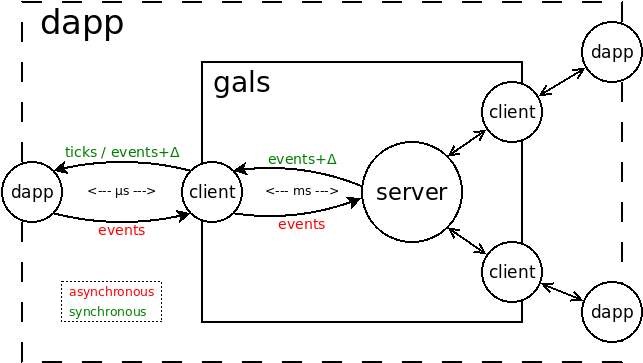
\includegraphics[width=\linewidth]{middleware}
  \caption{
    \label{fig.middleware}
    The architecture of the middleware \emph{gals}.
    A single server synchronizes multiple clients, each connected to a mirrored
    instance of the distributed application.
  }
  %\Description{A woman and a girl in white dresses sit in an open car.}
\end{figure}

The events represent user interactions, such as key presses, which are
unpredictable and need to be communicated with the other instances.
Since instances should be indistinguishable from one another, event sources are
irrelevant.
For instance, if a user presses a key in one instance, the \dapp behaves as if
all users pressed the same key in all instances simultaneously.
%
Clock ticks represent the rate in which applications are updated, and are
equivalent to frame rates in video playback and games.
For practical purposes, we assume periods in the order of tens of milliseconds
(e.g., 25 milliseconds or 40 frames per second).
An important insight is that clock ticks are predictable inputs and need not to
go through the server.
This results in no delay between the \dapp and the client since interprocess
communication takes negligible time (i.e., in the order of a few microseconds).
Unlike sporadic mechanical user input, clock ticks cannot tolerate considerable
delays without going unnoticed by humans.
%
Clock ticks and delayed events constitute the unique synchronous timeline
shared by all instances of the \dapp, allowing them to manifest identical
behavior.
Figure~\ref{fig.timeline} is an example of a timeline with asynchronous events
that are synchronized with a delay.
Except for inputs with event id \emph{0}, which reprepresent clock ticks, each
application determines its own ids, and the middleware just forwards them with
no processing.
As detailed in Section~\ref{sec.gals}, the middleware ensures that all
instances receive the same timeline.

\begin{figure}[t]
{\scriptsize
\begin{verbatim}
Tick    Event    Async
----    -----    -----
0000      0
0025      0      --> user presses key (1) and mouse (2)
0050      0
0075      0      --> user presses key (1)
0100      0
0125      1  <-- key is synchronized after delay
0150      0
0175      2  <-- mouse is synchronized after delay
0200      1  <-- key is synchronized after delay
0225      0
0250      0
....     ...
\end{verbatim}
}
  \caption{
    \label{fig.timeline}
    Example of a synchronized timeline of inputs shared by all instances of the
    \dapp.
    Ticks are \emph{25ms} apart (\emph{40 FPS}).
    Asynchronous events are synchronized with a delay.
    Note that delay is unpredictable but event order within each source
    instance is preserved.
  }
\end{figure}

%As detailed in Section~\ref{sec.gals}, the delta delay for user input is the
The delta delay for user input is the maximum network round-trip time
considering all clients.
We deliberately assume unbounded network delay to augment the scope of
applications.
Another concern is the rate of input generation in the instances.
As an example, tracking the mouse position will inevitably flood the network
with packets and make the application unresponsive.
For these reasons, the viability of applications depends on
    (i) the acceptable delay in the user input,
    (ii) the nature and rate of inputs, and
    (iii) the maximum network latency.

The code for an actual \dapp is the same for all instances and uses a standard
event-driven API with only four commands:
\begin{itemize}
\item \texttt{connect(port,fps)}:        \\Connects with the local client in the given port and desired FPS.
\item \texttt{disconnect()}:             \\Disconnects with the local client.
\item \texttt{(now,evt) = gals\_wait()}: \\Waits for the next input carrying a timestamp and event id.
\item \texttt{gals\_emit(evt)}:          \\Emits the given asynchronous input.
\end{itemize}
Figure~\ref{fig.skel} shows the skeleton of an application.
The commands \texttt{connect} and \texttt{disconnect} are only required once to
enclose the application logic.

\begin{figure}[t]
{\scriptsize
\begin{verbatim}
01  fun dapp (port: Int) {
02     gals_connect(port,40)          // connects to client at 40 FPS
03     while (true) {                 // main event loop
04        val (now,evt) = gals_wait() // awaits input (every 25ms)
05        switch (evt) {              // reacts to input
06           ...break loop...         //   possibly terminates
07        }
08        ...gals_emit(nxt)...        // possibly generates inputs
09     }
10     gals_disconnect()              // disconnects with the client
11  }
\end{verbatim}
}
  \caption{
    \label{fig.skel}
    The skeleton of a \dapp is a main loop that waits synchronous and emits
    asynchronous events.
  }
\end{figure}

Figure~\ref{fig.timeline}~and~\ref{fig.skel} with the timeline and the program
related as follows:
The application initially blocks at \emph{line 4} waiting for an input.
According to the timeline, the first input happens at \emph{tick 0} and
\emph{event 0} (no event).
In the second iteration \emph{tick 25}, the application emits events \emph{1}
and \emph{2} asynchronously at \emph{line 8}.
Only after a few ticks, these events are synchronized and awake \emph{line 4}
in subsequent ticks.
The main event loop is coded like a standard local event-driven application as
intended.

\section{Local Synchronous Programming}
\label{sec.sync}

In the synchronous programming model~\cite{sync}, a program executes in
locksteps (or logical ticks) as successive reactions to inputs provided by an
external environment.
In our context, the environment represents user interactions, and inputs can be
occasional events, such as a key press, or simply the passage of time.
Since execution is guided from outside, the main advantage of the synchronous
model is that it can record a sequence of inputs and reproduce the behavior of
a program multiple times for reasoning and testing purposes.
A fundamental requirement for synchronous programming, known as the
\emph{synchronous hypothesis}~\cite{hypo}, is to isolate logical ticks from one
another to preserve locksteps and prevent concurrent reactions to inputs, which
would break determinism.
This hypothesis is satisfied if computing reactions is faster than the rate of
external inputs.

An important concern is how to guarantee that isolated reactions are themselves
deterministic and sufficiently fast.
Synchronous languages~\cite{langs} typically restrict the programming
primitives and/or perform static analysis to ensure these properties.
However, since our solution proposes a standard event-driven API targeting
generic programming languages, we assume these properties are ensured
informally.
This may involve coding best practices like avoiding stateful system calls and
time-consuming loops.

\begin{figure}[t]
  \centering
  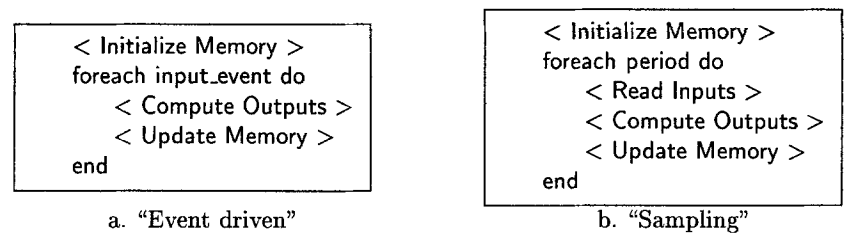
\includegraphics[width=\linewidth]{schemes}
  \caption{
    \label{fig.schemes}
    Equivalent execution schemes for synchronous systems~\cite{schemes}.
    In the first scheme, a change in the environment is designated as an input
    event. 
    In the second scheme, an instant is a predefined time interval in which
    the environment is polled for input events.
  }
\end{figure}

Figure~\ref{fig.schemes} shows two common implementation schemes for
synchronous systems~\cite{schemes}.
In both schemes, a loop iteration updates the state of the memory completely
before handling the next input.
Hence, assuming memory updates are deterministic, the only source of
non-determinism resides in the order of inputs from the environment.
Outputs are asynchronous events in the opposite direction of inputs and
signal the environment about changes.
They typically represent external actuators as opposed to input sensors.

The ``Sampling'' scheme of Figure~\ref{fig.schemes} is very similar to the
\dapp skeleton of Figure~\ref{fig.skel}:
    \texttt{gals\_connect} specifies the sampling period,
    \texttt{gals\_wait} reads inputs,
    \texttt{gals\_emit} signals the environment back, and
    the \texttt{switch} statement processes the inputs (to update memory).
As required by the synchronous hypothesis, the sampling period, and
consequently the rate of inputs, must be compatible with the processing speed.
A subtle particularity is that \dapps outputs are actually asynchronous inputs
later retrofitted back synchronized with a delay, as described in
Figure~\ref{fig.middleware}.
%
The sampling scheme is also adopted by popular event-driven libraries, such as
\emph{SDL} for computer graphics, and \emph{Arduino} for embedded systems.%
\footnote{\url{www.libsdl.org} and \url{www.arduino.cc}}
This allows for an easier integration of our middleware with practical systems,
and also reinforces how programming distributed versions are similar to their
local counterparts.

Figure~\ref{fig.sdl} is the code for a \dapp written in SDL to control an
animated rectangle on the screen with the keyboard.
The code structure follows the synchronous implementation scheme with well
delimited regions to initialize memory \lin{4--8}, read inputs in a loop
\lin{11--13}, update memory \lin{15--28}, and compute outputs \lin{30--31}.
As mentioned above, the outputs are actually asynchronous inputs that are later
retrofitted into the \dapp.
This region of code is expanded in Figure~\ref{fig.input} and is discussed in
sequence.
The application first initializes the SDL library to create a window and
renderer handle \lin{4--6}.
The rectangle starts at position \texttt{(10,10)} with no movement in the axes
\texttt{vx=vy=0} \lin{7--8}.
The main loop \lin{10--32} first waits for the next input to control the
rectangle \lin{11--13}.
On each iteration, the screen is cleared and the rectangle is drawn on the
current position \lin{15--19}.
The \texttt{switch} statement \lin{20--27} processes the current input:
    a clock tick \lin{21} just moves the rectangle in the current direction;
    a space \lin{22} pauses the rectangle by resetting the axes speeds;
    the arrow keys \lin{23--26} sets the axis speeds towards the appropriate direction.
Before the next iteration, the screen is updated \lin{28}.
The code is enclosed by middleware calls to connect and disconnect \lin{2,34}.
Inside the main loop, all state modifications depend only on the received
event, which ensures that the application is deterministic.

\begin{figure}[t]
{\scriptsize
\begin{verbatim}
01  int main (void) {
02    gals_connect(port, 40); // 25ms ticks
03
04    SDL_Init(SDL_INIT_VIDEO);                 ---\
05    SDL_Window*   win = SDL_CreateWindow();      |
06    SDL_Renderer* ren = SDL_CreateRenderer(win); |> Initialize
07    int x=10, vx=0; // position and              |    Memory
08    int y=10, vy=0; // speed multipler        ---/
09
10    while (1) {
11      uint64_t now;                           ---\
12      uint32_t evt;                              |> Read Inputs
13      gals_read(&now, &evt);                  ---/
14
15      SDL_SetRenderDrawColor(ren, WHITE);     ---\
16      SDL_RenderClear(ren); // clear screen      |
17      SDL_Rect r = { x, y, 10, 10 };             |
18      SDL_SetRenderDrawColor(ren, RED);          |
19      SDL_RenderFillRect(ren, &r); // draw rect  |
20      switch (evt) { // 5px/40fps -> 200 px/s    |
21        case 0:     { x+=5*vx; y+=5*vy; break; } |> Update Memory
22        case SPACE: { vy= 0; vx=0; break; }      |
23        case LEFT:  { vx=-1; vy=0; break; }      |
24        case RIGHT: { vx= 1; vy=0; break; }      |
25        case UP:    { vy=-1; vx=0; break; }      |
26        case DOWN:  { vy= 1; vx=0; break; }      |
27      }                                          |
28      SDL_RenderPresent(ren);                 ---/
29
30      // emit asynchronous inputs             ---\  Compute Outputs
31      ... gals_emit(evt) ...                  ---/
32    }
33
34    gals_disconnect();
35    return 0;
36  }
\end{verbatim}
}
  \caption{
    \label{fig.sdl}
    A \dapp in SDL to control an animated rectangle on the screen with the keyboard.
    Video with two running instances: \url{TODO}
  }
\end{figure}

Figure~\ref{fig.input} expands the output region with the calls to
\texttt{gals\_emit} that generate asynchronous inputs.
In this application, it simply calls the SDL library to check if a key is
pressed and forward to the middleware.
Note that in a local-only application this region of code would replace the
region to read inputs from the middleware.
Note also that it is not necessary to customize this code for every single
application.
Instead, the middleware may provide a custom input generation stub for each
event-driven library it supports, and \dapps may reuse it.
This is the reason why we split this code in a separate figure.

\begin{figure}[t]
{\scriptsize
\begin{verbatim}
// emit asynchronous inputs
SDL_Event inp;
if (SDL_PollEvent(&inp)) {
   if (inp.type == SDL_KEYDOWN) {
      switch (inp.key.keysym.sym) {
         case SDLK_LEFT:  { gals_emit(LEFT);  break; }
         case SDLK_RIGHT: { gals_emit(RIGHT); break; }
         case SDLK_UP:    { gals_emit(UP);    break; }
         case SDLK_DOWN:  { gals_emit(DOWN);  break; }
         case SDLK_SPACE: { gals_emit(SPACE); break; }
      }
   }
}
\end{verbatim}
}
  \caption{
    \label{fig.input}
    Asynchronous input generation with \texttt{gals\_emit}.
    The library polls for key presses and forwards them to the middleware.
  }
\end{figure}

To conclude this section, the ``Update Memory'' region of Figure~\ref{fig.sdl},
which contains the core logic of the application, does not make calls to the
middleware, being indistinguishable from a local version.
In addition, since this region complies with the synchronous model premises,
the application remains responsive and deterministic.
For instance, the computations to update the positions are clearly faster than
\emph{25ms} (a tick period), satisfying the synchronous hypothesis.
Also, if a given timeline such as that of Figure~\ref{fig.timeline} is
reproduced to the application, all intermediate and final values of \texttt{x}
and \texttt{y} will always be the same.
In the next section, we discuss how to extend these guarantees to a distributed
setting.

\section{Distributed GALS Architecture}
\label{sec.gals}

The synchronous programming model assumes a single clock that controls the main
loop to update the application state synchronously in locksteps.
However, when we distribute the \dapp in multiple instances, we can no longer
assume a single clock source, and we also introduce a delay in communication
that compromises the synchronous hypothesis.

Towards symmetric distributed applications with identical behavior, we need to
read inputs synchronized and in real time in all instances.
For instance, in the rectangle example of Figure~\ref{fig.sdl}, the challenge
is
    to awake all calls to \texttt{gals\_read} at the same time \lin{13}, and
    to broadcast and resynchronize all asynchronous calls to \texttt{gals\_emit} \lin{31}.

The ``Globally-Asynchronous Locally-Synchronous Architecture (GALS)''
integrates multiple independent synchronous processes as a single distributed
application~\cite{TODO}.
%
By adopting this architecture, we can keep the simplicity and guarantees of the
synchronous model to program local instances, and transfer the responsibility
to deal with asynchrony to the middleware at a global level.
%
In Figure~\ref{fig.middleware}, we can see that \dapp instances depend on
synchronous inputs only (green arrows), and are allowed to output asynchronous
events (red arrows), whose responsibility to resynchronize is left to the
middleware.

As introduced in Section~\ref{sec.arch}, resynchronization adds a delta delay
to the original event equal to the maximum network round-trip time considering
all clients.
The middleware synchronization algorithm needs to consider two main problems:
%
\begin{itemize}
\item \textbf{Clock differences:}
    Each instance has an independent clock that differs from others in the
    \emph{offset} and \emph{rate}.
    The offset refers to the point in time since the \dapp started.
    As an example, one instance started \emph{5000ms} ago while another started
    \emph{5051ms} ago.
    The \emph{rate} refers to the how fast the clock progresses, which may
    slightly differ between machines.
    As an example, one instance misses \emph{25ms} every hour in comparison to
    others.
    This difference, aka \emph{clock drift}, may affect the time offset
    considerably over time.
\item \textbf{Network delay:}
    The instances carry a communication delay with the server, which varies
    between clients and also over time.
    As an example, a client next to the server may have a consistent RTT of
    \emph{10ms}, while a distant one may vary between \emph{50--100ms} over
    time.
\end{itemize}
%
We do not assume any strict timing bounds in our synchronization algorithm,
which may of course affect the viability of some applications.

The synchronization algorithm performed by the middleware has the following
objectives:
%
\begin{enumerate}
\item Keep the instances clock offsets close to each other.
\item Generate synchronous inputs to instances with a minimum delay.
\item Ensure that instances read the inputs with perfect time precision.
\end{enumerate}
%
Regarding \emph{goal 1}, offset differences are inevitable but should be under
a few milliseconds to not be perceived by users.
Regarding \emph{goal 2}, the smaller is the input delay, the better is the user
experience regarding interactivity.
However, if too small, a distant instance may nevertheless receive the delayed
input after its local time, which is unacceptable considering \emph{goal 3}.
In this case, the middleware may freeze the instance and pause its local time
to ensure time precision.

Figure~\ref{fig.protocol} describes the synchronization protocol performed by
the middleware.
The next paragraphs explains the protocol in detail.

The server starts first and needs to know in advance how many instances will
participate in the \dapp (\emph{Server (N)}).
Each instance connects through its client (\emph{Client 1 ... Client N}) with
the server, which waits for all connections to succeed (\emph{all connected}).
Then, the server broadcasts a \emph{start} message to all clients, which on
receipt, starts to send ticks to their instances (\emph{started}).
Note that clients will inevitably start at different global times due to
network latency.
The clients also send back an \emph{ack} so that the server can calculate the
maximum network RTT1 (\emph{45ms}), which is used next.
%
After the startup process, each \dapp instance executes at the same pace
(except for drifts) with similar offset differences (under maximum RTT1).
We consider that, at this point, the instances are indistinguishable from each
other.

\begin{figure}[t]
  \centering
  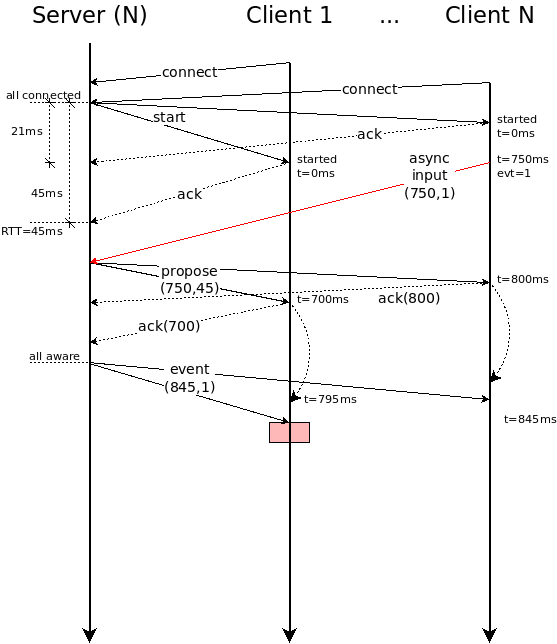
\includegraphics[width=\linewidth]{protocol}
  \caption{
    \label{fig.protocol}
    The architecture of the middleware \emph{gals}.
    A single server synchronizes multiple clients, each connected to a mirrored
    instance of the distributed application.
  }
  %\Description{A woman and a girl in white dresses sit in an open car.}
\end{figure}

Now, let's consider an asynchronous event: \emph{Client N} emits event \emph{1}
at local time \emph{750ms}.
The server enqueues all event requests (in red) and handles each atomically, in
sequence, as described further.
%
Note that the client cannot determine a reasonable timestamp for the event and
broadcast it directly to others.
First, the client has no idea about the network RTT to propose a deadline
timestamp (e.g, \emph{750+RTT}) that guarantees that all clients receive the
event in time to fulfill \emph{goal 3}.
Second, even if known, there is no guarantee that the RTT will not slightly
increase this time, making an instance to miss the event deadline.
Third, even if the RTT was known and bounded, the local instances may still
diverge on their local time offsets (e.g., \emph{750ms} vs \emph{800ms}), again
making an instance to miss the deadline.
%
As mentioned above, we do not assume any bounds in RTT and offset variance.

Hence, our protocol relies on the server to determine a reasonable timestamp
for all clients, and to ensure that instances do not miss the deadline even if
everything goes wrong.
%
First, the server broadcasts the intention to emit an event, passing the source
instance offset time and current network maximum RTT1 (\emph{propose(750,45)}).
The final confirmation of the event is yet to come after all clients
acknowledge the server (\emph{event(890,1)}).
Before that, each client calculates its own deadline as follows:
    (i) take the maximum time between the source and local offset,
    (ii) add twice the received RTT to this maximum, and
    (iii) set this sum as the local event deadline.
As examples, the sum for
    \emph{Client 1} is $max(750,700)+2x45=840$, and for
    \emph{Client N} is $max(750,800)+2x45=890$.
%
This sum is reasonable because it considers
    the instance most ahead in time, and also
    the worst RTT with an extra margin.
For instance, \emph{Client N} with the worst RTT (\emph{45ms}) is also ahead of
time \emph{800ms} and the final confirmation will arrive after another round
trip to the server (\emph{event(890,1)}), making \emph{890ms} a reasonable
deadline.
%
During this process, the server recalculates the RTT to use in the next event
emission (\emph{RTT2=50ms}).

Each client also starts a timer to pause the instance if the confirmation of
the event is not received until the deadline.
In this case, the client pauses the instance by repeating the same tick over
and over until it receives the now expected event.
This at least ensures identical timelines in all instances of the \dapp.
%
The server then wait for all client acknowledgments carrying their local
offsets (\emph{ack(800)} and \emph{ack(700)}), recalculate each deadline (in
the same way each client did), and takes the largest as the final event
timestamp to broadcast to all clients (\emph{event(890,1)}).
The server also sends a drift compensation (\emph{dt(0)} and \emph{dt(100)})
based on offset differences, which is discussed further.
At this point, all clients are expecting a timestamp that is greater than or
equal to their own timer deadlines.
Therefore, even if the network deteriorates, no instances can miss the
synchronized event.

Finally, the final confirmation is received by the clients.
\emph{Client N} receives it before the deadline, at local time \emph{870ms},
which requires to postpone local emission for \emph{20ms}.
However, \emph{Client 1} expires its timer before receipt and needs to pause
the \dapp for a while (red area).
Then, the event confirmation is received at local time \emph{860ms}, but which
still requires to postpone local emission for another \emph{30ms}.
In the end, both clients emit the event exactly at local time \emph{890ms} as
expected (white circle in the Figure).

Note that \emph{Client 1} was harmed in the process mainly because the maximum
time it used (\emph{750ms}) was much smaller than \emph{Client N} did
(\emph{800ms}).
This is because the local clocks were too distant from each other, breaking our
\emph{goal 1}.
As an additional remark, note that pausing \emph{Client 1}, increased the
offset difference even further (\emph{offset diff} in the Figure).
%
The middleware also implements an algorithm to compensate clock drifts as
follows:
Once the server receives all acknowledges carrying local offsets
(\emph{ack(800)} and \emph{ack(700)}), the server sends back how much each
client is delayed it in comparison to the maximum value (\emph{0} and
\emph{100}).
If the number is greater than zero, the client speeds up each instance tick in
\emph{20\%} until the time drift is compensated.
For instance, if the client generates new ticks every \emph{25ms}, it will
instead generate a new \emph{25ms} tick every \emph{20ms}.

\begin{comment}
With distribution, communication timing is asynchronous because communication
latency takes a non-negligible time and breaks the synchronous hypothesis.

Test locally in one instance is the same as N instances in M machines
What about in realtime
- a perfect mirror, cannot distinguish
- high-level vs low-leve events, semantic events
    - more abstract solves both problems (delay and rate)
- clear/sound properties to reason
- Events: single application, multiple views, may restrict events per node

Concurrent programs in non-deterministic languages are notoriously hard to prove correct and have led to well-known disasters.
\end{comment}

\section{Evaluation}
\label{sec.eval}

% - asymmetric, different view, multiple inputs
% - what ifs c/ videos
% - revisitar limitacoes e propor alternativas na secao de avaliacao
% - Every five seconds one client generate a tick To update rtt and keep pace

\section{Related Work}
\label{sec.related}

\begin{comment}
Asynchronous languages and models:

Derflow: distributed deterministic dataflow programming for erlang
Erlang implements a message-passing execution model in which concurrent processes send each other messages asynchronously. This model is inherently non-deterministic: a process can receive messages sent by any process which knows its process identifier, leading to an exponential number of possible executions based on the number messages received.
We propose a new execution model for Erlang, ''Deterministic Dataflow Programming'', based on a highly available, scalable single-assignment data store implemented on top of the riak\_core distributed systems framework.

Deterministic Actors
While actors provide a more disciplined model for concurrency than threads, their interactions, if not constrained, admit nondeterminism.
 We describe “reactors,” a new coordination model that combines ideas from several of the aforementioned approaches to enable determinism while preserving much of the style of actors.

Deterministic replay of distributed Java applications
Execution behavior of a Java application can be nondeterministic due to concurrent threads of execution, thread scheduling, and variable network delays. This nondeterminism in Java makes the understanding and debugging of multi-threaded distributed Java applications a difficult and a laborious process.
It is well accepted that providing deterministic replay of application execution is a key step towards programmer productivity and program under-standing.
Towards this goal, we developed a replay framework based on logical thread schedules and logical intervals.

Synchronous languages and models:

A Programming Model for Time-Synchronized Distributed Real-Time Systems
Discrete-event (DE) models are formal system specifications that have analysable deterministic behaviors. Using a global, consistent notion of time, DE components communicate via time-stamped events.
In this paper, we extend DE models with the capability of relating certain events to physical time.
Our technique relies on having a distributed common notion of time, known to some precision.
\end{comment}

\section{Conclusion}
\label{sec.conclusion}

\bibliographystyle{ACM-Reference-Format}
\bibliography{rebls-21}

\end{document}
\endinput
